\chapter{Introduction}

\section{Environmental Pressures and Aviation Technology}
\indent The current trend in industry standards for aviation technology is towards technologies with more fuel efficient and less noisy vehicles and power systems. Many entities including government agencies such as NASA and the FAA are interested in studying the effects of specific technologies to assess the potential return on investment of the technology to properly appropriate scarce government research dollars. In this context, many technologies require reasonable assessments of improvements at the conceptual level, when much design information is utterly lacking.  In many cases, the technologies of interest are new materials, which may simply require refinement of the manufacturing processes required to achieve the necessary material strengths and thermal properties. Other types of technologies are related to the design of specific components which improve efficiencies, decrease losses, or improve operability and durability throughout the component lifetime. Another class of technologies are those which alter the aerodynamics of the vehicle, such as winglets, ribs, or boundary layer laminar flow control. Such technologies are more dependent on the design of the vehicle and require proper design of the technologies. The environmental benefits of these technologies thus rely upon having reasonable design methods to assess their potential improvements.  One such technology which falls into the latter class and is the subject of this thesis is boundary layer ingestion, or "BLI" for short. Rather than being a "technology", it is instead a novel arrangement of the propulsion system such that it interacts positively with the aircraft wake to produce higher propulsive efficiencies. This is done by at least partially embedding the engine into the aircraft surface and ingesting the low-momentum boundary layer flow into the propulsor. Ingesting the boundary layer is beneficial because of the natural tendency for turbomachines, such as a fan, to do more work on sections of the flow with lower total inlet pressure \cite{Smith1993}.  BLI therefore has the effect of re-energizing the aircraft wake thereby reducing total drag relative to an aircraft with podded engines and improving the propulsive efficiency of the system.  NASA has identified aggressive fuel burn targets for the next generation of aircraft and beyond as shown in figure \ref{Fuel_Burn_Targets}.  Boundary layer ingestion has been identified as a potential technology to help enable the achievement of these fuel burn targets.  


\begin{table}[ht]
\caption{NASA fuel burn targets for the next generation of aviation vehicles. \cite{Kestner2011}}
\centering
\begin{tabular}{cc}
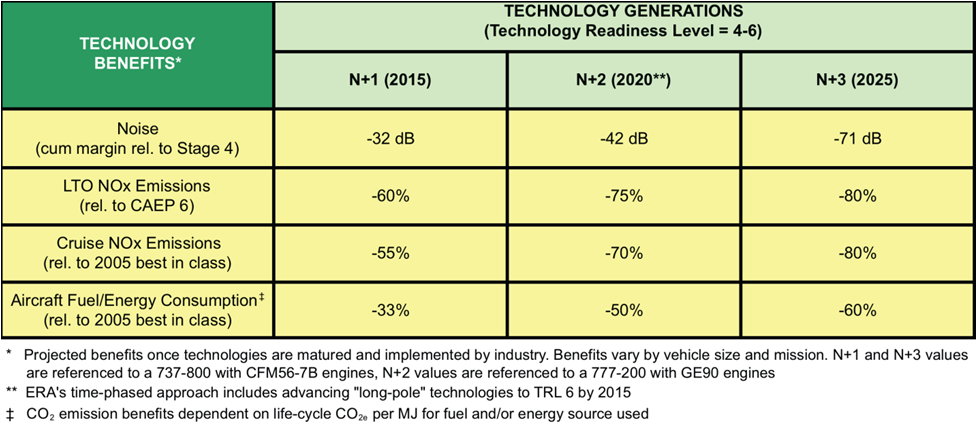
\includegraphics[width=120mm, height = 70mm, trim=0mm 0mm 0mm 0mm, clip=true]{Fuel_Burn_Targets.png}
\end{tabular}
\label{Fuel_Burn_Targets}
\end{table}


\section{Boundary Layer Ingestion}
Boundary layer ingestion (BLI) has been known and practiced within maritime engineering for quite some time now. The main effect comes from the propulsive efficiency gains from ingesting the low-momentum flow into the propulsor and re-energizing the flow to a velocity much higher than it would be otherwise, thereby reducing the overall propulsive power required to overcome the dissipative forces acting on the vehicle. In aviation, the gains from BLI are theoretically plausible and have been studied at some length but have yet to come to fruition in civil applications due to the additional difficulty of designing a proper aerodynamic intake which can deliver reasonable levels of distortion to the fan and compression system at transonic flight speeds and Reynold's numbers. However, the next generation of aircraft may have much better performance synergy with the integrated propulsive systems such that the costs of designing to negate the impacts on the engine operation of BLI are offset by the reduction in fuel consumption. One such futuristic aircraft which synergizes well with the BLI concept is the hybrid wing body. The synergy with BLI arises from the large space on the upper surface of the aircraft which is available for the placement of engines within the airframe. There are other aircraft configurations for which BLI could be a plausible option, including the "double bubble" aircraft, which is an aircraft resembling a conventional tube and wing aircraft but with a significantly flatter and wider body on the upper surface allowing for 2 or 3 embedded BLI engines. In fact, the configuration is such that almost the entire upper fuselage boundary layer can be ingested into the engine, which is a relatively large percentage of the total vehicle drag.  There are various possibilities for propulsion system configurations which may include BLI. These possibilities include but are not limited to distributed propulsion, embedded, or flush-mounted. A distributed propulsion system is a system with many small propulsors "distributed" over the upper surface in an array type configuration.  This type of system is synergistic with BLI for reasons to be explained later in this chaper. The embedded and flush mounted configurations refer to the relative position of the engine compression face centerline with respect to the inlet highlight centerline. The embedded system has an "S-Duct" which guides the flow to the engine compression system situated lower in the airframe. The "flush-mounted" system has the engine flush with the aircraft surface meaning that the wetted area of the nacelle cowl would be slightly larger than the embedded case.  Among these configurations, there are multiple engine architectures which are possible including traditional turbofan direct-drive engines, geared turbofans, single-core/multi-fan type systems (e.g. tri-fan).  The single-core/multi-fan type systems have the benefit of being able to ingest much more boundary layer while avoiding the negative impacts on the gas turbine core.  Any design method for BLI systems must be able to include the physical performance differences between these engine congurations as well as the system weight and mission analysis to determine fuel burn for the entire system.

\subsection{BLI Benefits}
The benefits of BLI can be described, in principle, as a reduction in the total power requirement of the vehicle due to the increase in propulsive efficiency.  Additionally, the weight of the propulsion system is typically improved because of the elimination of the need for an engine pylon. There is also a nacelle wetted area reduction since the pylon and nacelle wetted area is less with the embedded or flush mounted engines having some of their surface area contained within the aircraft and not wetted by the air.  Lowering the engine closer to the airframe also incidentally has the effect of improving the pitch control of the aircraft with the thrust vector momentum arm being smaller.  

\indent Figure \ref{Podded_vs_Embedded_Engines} illustrates the basic difference between an ideal BLI engine and a podded engine \cite{PlasThesis}.  Here U$_\infty$ represents the free-stream velocity and $U_w$ represents the averaged wake velocity in the podded case. From classical propulsion theory, the input power required is given by equation \ref{Power_Added_Podded} for the podded case and by equation \ref{Power_Added_BLI} for the BLI case, where Uj is the jet velocity exiting the nozzle and is assumed to be the free-stream velocity in the BLI case.
    \begin{figure}
    \centering
    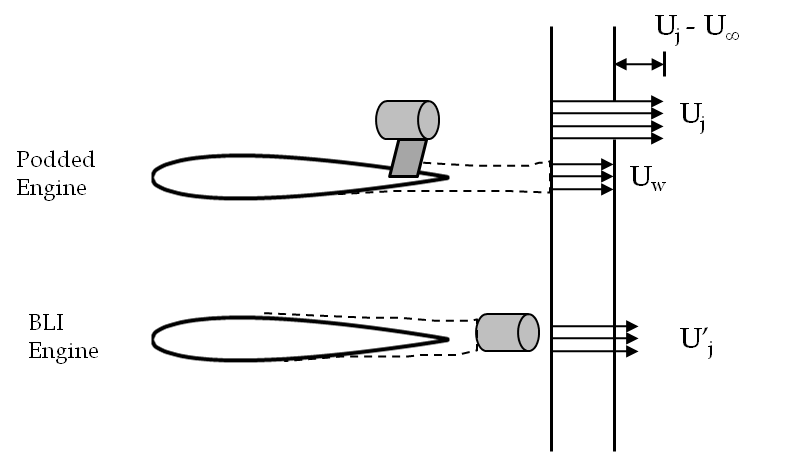
\includegraphics[width=140mm, height = 80mm, trim=0mm 0mm 0mm 0mm, clip=true]{Figure1_Podded_vs_Embedded_Engines.png}
    \caption{Notional diagram of podded vs. BLI engine design}
    \label{Podded_vs_Embedded_Engines}
    \end{figure}
\begin{equation}P_{Podded}= \frac{\dot{m}}{2}\big(U_j^2-U_\infty^2\big) = \frac{F_{n Podded}}{2}\big(U_j+U_\infty\big)\label{Power_Added_Podded}\end{equation}
\begin{equation}F_{n Podded}= \dot{m}\big(U_j-U_\infty\big) \label{Net_Thrust_Podded}\end{equation}
\begin{equation}P_{BLI}= \frac{\dot{m}}{2}\big(U_j^2-U_w^2\big) = \frac{F_{n BLI}}{2}\big(U_j +U_w\big)\label{Power_Added_BLI}\end{equation}
\begin{equation}F_{n BLI}= \dot{m}\big(U_j-U_w\big) \label{Net_Thrust_BLI}\end{equation}
Since $U_w$ is inherently less than the jet velocity, comparing equations \ref{Power_Added_Podded} and \ref{Power_Added_BLI} shows that the power required for the BLI case is less than for the podded case.  Although this is the simplest idealization of BLI, this is sufficient to explain the basic physics.  Because of the aero-propulsion interaction, the total benefit of the system is dependent on the propulsion system arrangement and the incoming airframe wake at the intake location, thus leading to the large disparity in possible benefit. 
\subsection{BLI Risks}

Perhaps the most significant risk with regard to BLI is the performance of the inlet and fan system.  The intake of an aircraft engine, while simple, is an absolutely essential component whose performance has a high impact on the specific fuel consumption of the engine.  The intake must supply the necessary amount of air flow to the compression system to accomodate the required level of thrust without significant losses or flow distortion which can lead to performance degradation or compression stability concerns. Two risks arise from this problem: 1.) inherent uncertainty in engine performance (related to inlet total pressure recovery and fan distortion); 2.) Compromised stability of the compression system due to the presence of both steady-state and dynamic inlet total pressure and swirl distortion.  In other words, there is a risk that the BLI induced gains in propulsive efficiency may be offset by the presence of a poorly performing inlet configuration and also risk that the engine, while more efficient, might simply not be operable over the required flight envelope of a civil air transport. Nichols, in an evaluation of the Silent Aircraft Initiative, also identifies these risks as the primary factors of uncertainty for the concept.  

There are other ancillary risks such as the effect of the distortion on component degradation and lifetime. Such factors can significantly impact operability costs and potentially offset some of the fuel burn cost savings. There is also the additional difficulty of designing a system which has a highly integrated airframe and propulsion system. This concern is exacerbated by the fact that these components are produced by separate companies requiring the need for intercorporate cooperation to certify this new technology and provide for an economical design. There are also other detailed factors such as the control of a system which is specifically designed to have steady-state and transient turbulent distortion present during operation or vibration which might arise from the same phenomenon. Significant research funding has gone into investigating the possibility of designing a "distortion tolerant fan" which can operate under the types of distortion related to BLI with improved efficiency and stall margin. However, this possibility remains uncertain as the research is still in progress.

\section{Design Methods}
Before talking about the methods of engine design with BLI, it is worth discussing some general design terminology and concepts. Broadly speaking, there are 3 primary phases of the design process: conceptual, preliminary, and detailed. The conceptual design phase is the very earliest phase in which system requirements, architecture, and basic performance characteristics are formulated. Preliminary design moves the system towards a more concrete physical definition by giving some of the components geometric definition, and initial conceptual performance estimates are modified in light of the new design information. Detail design is logically the next phase in which every single detail of the design is decided up to the point where manufacturing takes place. This last phase is the most involved, most expensive, and therefore the most costly should errors in the process necessitate design changes. Recent advances in design over the course of the last few decades have transitioned towards including elements of the latter two design phases in the conceptual phase using higher-order physics based tools to estimate detailed design performance. This is really happening because some of the newer technological concepts require detailed design understanding and quantification in order to determine the feasibility of the technology up front.  BLI is certainly a great example of where this design paradigm is most appropriate, since the propulsion design essentially depends upon the characteristic of the engine intake and the thrust requirement coming from the vehicle aerodynamics and flight conditions, thus lending itself to higher fidelity multi-disciplinary methods.  Conceptual design is the most important phase in the design process, especially for complicated systems with many subsystems.  Early design mistakes due to large uncertainty in performance or system feasibility can have large influence on costs later in the design phases, since all component designs depend on conceptual design choices. As such, changes in the conceptual  design of the system can have critical consequences if made in the detail phase and are amplified as the product matures.  

In the case of newer technologies which are unproven and highly uncertain, the need to minimize uncertainty and maximize the probability of success of the technology when integrated into a system is especially high. This can be difficult since technologies are not only expected to be able to maintain current state of the art capability but to improve upon it substantially to justify the additional research expenditures and investment involved in it's development.  Potential customers need to know that the product will be as reliable as their current technology but will offer additional operability cost savings to justify new purchases. If the technology benefits are not proven to customers or are shown to be negative, then the aircraft program could stand to be cancelled leading to large lost cost.  


\subsection{Conceptual Architectural Studies}
There are a number of conceptual design methods for propulsion systems in use today. The most common, at least at the conceptual level, is the thermodynamic cycle analysis. Typically these are "0-D", axisymmetric analyses that aim to provide thermodynamic gas path properties, thrust, and fuel flow. This type of analysis typically requires some characterization of each component of the propulsion system (from compression systems to the intake, nozzles, ducts, and combustors).  Cycle analysis is done in two modes: on-design and off-design. In on-design, the engine is sized to meet specific thrust targets at a given flight condition(s). In off-design, the performance of the engine is determined at other ambient conditions that are not considered the design condition. The final product of this analysis is engine thrust and fuel flow as a function of mach number, altitude, and throttle (power code). This is typically called the "engine deck". This information is used in the aircraft sizing and synthesis analysis to determine total take-off gross weight and mission fuel burn. In this way, changes in engine design or technology can be mapped to the system level through physical analysis.  Recent advances in cycle modeling tools have made "multiple-design point" on-design cycle analysis possible. This is the process of simultaneously satisfying multiple thrust targets and constraints at various conditions, whereas traditional single-point design only considers one. This is necessary because propulsion systems need to satisfy thrust requirements at various flight conditions such as top of climb (TOC), cruise, take-off (TKO), and sea-level static (SLS). Many studies focusing on BLI tend to only include the cruise or SLS conditions as the thrust sizing points when doing the on-design cycle analysis, which is really inadequate. More details will be given in chapter 2 on the MDP cycle analysis process and how it might be used with BLI.  For BLI, there have been many studies which involve the use of cycle analysis, even though modeling BLI requires some way of representing the non-uniform flow.  One way of doing this is to simply mix (average) the flow. This leads to certain errors in performance estimates since averaging the flow in this way tends to violate one conservation law or the other (mass, momentum). There are other methods of modeling the impact of BLI on cycle performance which resolve this difficulty such as the parallel compressor model, which is a "1-D" analysis and tends to better capture the impact on fan efficiency and stall margin. More complicated methods can also
predict the distortion transfer across the fan which can have an impact on the final performance.  Many of the studies that have implemented these types of 0-D or 1-D analyses are intended to give a first order estimate of fuel burn benefit. These estimates are used for architectural trade studies to determine the number of engines, engine placement, engine cycle, and other engine parameters. Typically higher order analyses are required for determining the detailed design of the inlet and external cowl shape, but such analyses require a cycle model to create boundary conditions for the computational analysis. A parametric cycle model also allows up-front sensitivity studies on the CFD analysis results.

\subsection{High-Fidelity Integration Studies}

There is another basic type of study which is common in the BLI literature which relate more to the detailed design of the inlet configuration. These are typically done to design the shape of the inlet diffuser and external cowl based on computational fluid dynamics. The objective of these are to reduce inlet distortion and total pressure loss, and to get better estimates of the total drag of the vehicle with the integrated engine.  These details are very important to the quality and performance of the design, but are additionally very expensive to obtain because BLI requires some level of viscous analysis (typically RANS) and is subject to separation effects which can require very refined grid sizes. Higher order studies tend to be more computationally expensive than the simpler 0-D or 1-D estimates which means that the designer should have aviable choice of propulsion system architecture and engine cycle before going to the detailed higher-fidelity phase. Spending limited computational resources on shape optimizing an inlet for a sub-optimal configuration is obviously undesirable.

\section{Need for a Propulsion Systems Design Framework}

\indent As such, the design process must involve designing to maximize the influences of the benefits and reduce the influence of the risks as economically as possible. In the case of BLI propulsion systems, this requires appropriate choice of architecture, component designs, engine type, and many other factors all of which affect the technology "benefit". BLI surely offers a design benefit in theory, but its presence is so physically significant that it necessitates changes in the way that the engine and airframe are designed to ensure system viability. It is not simply something that can be added to any design and be expected to yield a high confidence benefit, which is part of what makes this a challenging and interesting problem.
\indent A recent report by Boeing and NASA state that the BLI technology is currently "TRL 2" \cite{Bradley2012}.  Technology readiness level, or TRL, is a qualitative measure of how ready or proven a given technology is for practical usage.  The study states that the current state of the technology includes \cite{Bradley2012}:
\begin{itemize}
\item{Concepts for reducing distortion have been studied.}
\item{Some BLI configurations have been conceived.}
\item{Some studies have shown benefits for BLI.}
\end{itemize}

To mature the technology to TRL 3, the maturation plan for BLI is stated as:

\begin{itemize}
\item{A conceptual BLI aircraft configuration will be developed as a focal point for more detailed
development and as target for assessment of system-level benefits.}
\item{A BLI engine installation will be designed and analyzed with goals of ingesting substantial
boundary layer flow while keeping the boundary layer flow away from the engine core.}
\item{Approaches for reducing distortion from ingested boundary layer flows will be analyzed.}
\item{The BLI aircraft aerodynamic lines will be adjusted for the BLI engine installation.}
\item{Aerodynamic analysis of the integrated BLI configuration will be performed for cruise and
significant off-design conditions.}
\item{BLI-compatible engines will be designed for best efficiency given the anticipated engine flows.}
\item{A concept for BLI engine structural integration will be developed and analyzed.}
\item{A system-level assessment of the benefits of BLI will be made from the results of the analysis
studies.}
\end{itemize}

Note that the second bullet in the above list is the selection of a BLI installation for ingesting maximum boundary layer.  The following bullets then discuss the potential tactics for battling the inlet distortion, improving aerodynamic efficiency, and finally designing an engine which maximizes efficiency given the aerodynamics of the configuration.  The problem with this design process is that the initial analysis which determines the BLI engine installation will need to account for some of the information which is to be defined in later steps.  This provides the basic motivation for a conceptual, physics based, system level analysis tool which can account for uncertainty in the inputs to the system level model.  As such, the primary research objective for this dissertation is as follows:

\vspace{25pt}
\fbox{
  \parbox{\textwidth}{Primary Research Objective:  Develop a methodology for conceptual system level analysis of BLI propulsion systems which can allow for simultaneous satisfaction of system requirements and constraints at multiple design conditions, quantify BLI performance impacts, determine critical design conditions, and quantify sources of uncertainty and their relative contribution to variation in the system metrics of interest and select a design which is robust to uncertainty.  
}
}
